%!TEX root = ../thesis.tex
%*******************************************************************************
%*********************************** First Chapter *****************************
%*******************************************************************************
%The first big part is the introduction. It may seem similar to an abstract. It pursues different goals –reader hooking, providing background information and logical transition to your own research. Here is what you need to disclose in this chapter:

%Enough background information about previous researches should be presented to make readers understand place of text in science system.
%Give an explanation concerning contents – what will be included into thesis.
%Provide readers with verbal ‘road maps’.
%Cite previous works. The citations must be related to text’s goals. Do not list everything you have read about subject.
%These sections must take three pages of paper, excluding contents and table lists.

\chapter{Introduction}  %Title of the First Chapter
%********************************** %First Section  **************************************
Today the world is witnessing an exponential increase in camera deployment ~\citep{ananthanarayanan2019demo} with cities and organizations steadily increasing the size and reach of their deployments. For example, cities now deploy tens thousands of cameras, each continually collecting and strreaming rich video data \cite{ref0}, \cite{ref1}, \cite{ref2}. According to IHS Markit’s annual report \cite{oliverreport}, as of 2018, China has one camera for each 4.1 people in the country and the United State has a people-to-camera ratio of 4.6-to-1. The massive deployments of cameras are brought on mainly by the growth of the video surveillance industry due to increasing concerns about public safety and security. With such prevalent trend, intelligent video analytics systems have been playing an essential role, performing important task in various fields including surveillance, transportation, manufacturing, etc. These systems analyze video feeds to guide long-running tasks such as traffic monitoring, customer tracking, and surveillance. Key to the success of such applications has been recent advances in computer vision, particularly neural network based techniques for highly accurate object detection and recognition \cite{cai2015learning}, \cite{krizhevsky2017imagenet}, \cite{li2015convolutional}.\\
In a typical real-time video analytics pipeline as 
\begin{figure*}
\centering
 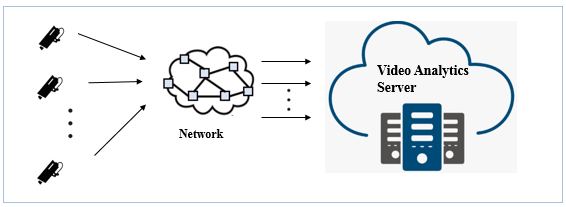
\includegraphics[width=1.0\linewidth]{Figures/cloud.png}
 \caption{Overall of cloud based video analytics server}
 \label{fig:overall}
\end{figure*}
Figure \ref{fig:overall} illustrates a traditional cloud-based video stream analytics system. A large number of camera transfer video data to a central cloud (datacenter) where video analytics is performed. However, this traditional approach makes it difficult to perform real-time analytics on live video streams from many cameras because the video analytics involves several computation-intensive tasks such as object detection, object tracking, object recognition and so on. Besides, streaming video from multiple camera to the cloud consumes a lot of network bandwidth over limited-bandwidth networks, which leads to high latency, causing significant challenge for real-time video analytics.\\
Significant work has been expended to improve the efficiency of video analytics pipelines \cite{canel2019scaling}, \cite{chen2015glimpse}, \cite{hsieh2018focus}, \cite{jiang2018chameleon}. Accross these systems, a prevailing (and natural) strategy is to improve efficiency by filtering out frames that do not contain relevant information for the query. Conceptually, filtering out a frame would affect a query result. In this study, to address addresses the question of how to overcome this network bottleneck and offload large volumes of data from a distributed camera deployment in real-time to a datacenter for further processing, we aim to develop a solution by harnessing edge computing. \\
Video analytics at the edge has multiple benefits such as decreasing the response time, saving network bandwidth, and minimizing the peak workload to the cloud. However, edge devices are typically much less powerful than the cloud, with limited computing resources such as a few GPUs (graphics processing units) and CPUs (central processing units), as well as smaller RAM (Random Access Memory) capacities \cite{stone2019towards}. In the field of public safety, the ability to simultaneously process multiple feeds and provide real-time video analytics is critical. Therefore, this study seeks to answers how edge devices and the cloud can cooperate in an efficient manner to achieve real-time and scalable video analytics.  \\
One of the features frequently observed in surveillance camera images is that captured images remain unchanged for a long time and video content is often quite redundant. Therefore, it is undesirable to conduct analytics on redundant video frames from cameras, leading to a waste of computing resources and power consumption in the cloud. Motivated by this, we propose a pre-process module that acts as a video filter function at the edge device to eliminate the redundant static images before feeding videos to the cloud for further analysis. The proposed method runs on an edge device and recognizes the motions (i.e., moving objects) in the consecutive video frames. Based on the motion recognition result, our module decides whether to pass the video frame to the cloud or filter it out. As a result, the proposed motion-based filtering module can reduce not only computational load of the cloud nodes but also network traffic to the cloud. \\
Motion recognition schemes can be classified into two categories: (i) video pixel-domain based and (ii) video compressed-domain based approaches. In pixel-domain based approaches \cite{lu2014moving}, \cite{kumar2016segmentation}, \cite{gujrathi2014detecting}, \cite{wang2019ground} video is completely decoded before using background modelling or vision based deep learning framework to detect moving objects at the pixel level. The performance of video pixel-domain processing in large systems may be challenged by the load of decoding multiple streams and the image pixel-based calculation. Thus, pixel-based approach requires higher computational complexity and can make it difficult to fulfill the real-time requirement of edge devices. 
Compressed-domain approaches \cite{favalli2000object},\cite{yoneyama1999moving},\cite{dong2006object},\cite{achanta2002compressed} rely on video coding artifacts of compressed bitstreams such as motion vector (MV), macroblock partitions, and quantization coefficients for recognizing motion. Compared to pixel-domain based algorithms, compressed-domain methods generally require less computational resources because analyzing input information is already possible in the bitstream.\\ In this study, we proposed a compressed-domain based moving objects detection that applies a data clustering and an intersection of union (IoU) rate-based object tracking technique of computer vision. Using only MVs, which are provided by video encoders in a compressed bitstream, our approach is able to efficiently detect moving objects. Furthermore, an experimental evaluation of our method is provided to compare it with the state-of-the-art compressed-domain tracking methods in term of processing time, and demonstrate its functionalities to evaluate the efficiency of the proposed edge device with a cloud video analytics server in a real-world scenario. In summary, this paper makes the following contributions.
\begin{itemize}
\item Introduction of a compressed-domain moving objects detection method that can be applied for numerous surveillance applications.
\item Design an edge-to-cloud computing system for surveillance video analytics that applies the proposed method at edge devices to minimize the transfer of video data from surveillance camera feeds to the cloud.
\item Implementation and evaluation of the proposed method with an edge-cloud system. The implementation is lightweight and easy to deploy at any edge devices.
\end{itemize}
%
\nomenclature[z-VMS]{VMS}{Video Management Software}
\nomenclature[z-VA]{VA}{Video Analytics}
\nomenclature[z-CCTV]{CCTV}{Closed Circuit Television}
\nomenclature[z-CNN]{CNN}{Convolutional Neural Networks}
\nomenclature[z-FPS]{FPS}{Frames Per Second}
\nomenclature[z-MV]{MV}{Motion Vector}
\nomenclature[z-AVC]{AVC}{Advanced Video Coding}
\nomenclature[z-RTSP]{RTSP}{Real-Time Streaming Protocol}
\nomenclature[z-MCP]{MCP}{Motion-Compensated Prediction}
\nomenclature[z-HEVC]{HEVC}{High Efficiency Video Coding}
\nomenclature[z-R-CNN]{R-CNN}{Regions with CNN}
\nomenclature[z-SSD]{SSD}{Single Shot Multi-box Detector}
\nomenclature[z-YOLO]{YOLO}{You Only Look Once}
\nomenclature[z-CPU]{CPU}{Central Processing Unit}
\nomenclature[z-GPU]{GPU}{Graphics Processing Unit}
\nomenclature[z-RAM]{RAM}{Random Access Memory}
\nomenclature[z-CUDA]{CUDA}{Compute Unified Device Architecture}
\nomenclature[z-IOU]{IoU}{Intersection Over Union}
%